% \section{Abstract model for DAE units}

It is better to draw easier-to-understand pictures. Explanation: \ldots Call those DNA sequences ``glues''.

In following examples this model will be set up to act similarly like NP: $\exists y \; R(x,y)$. Although existence is not sure, it is very likely. Predicate $R$ will be ``enumerable in polynomial time'' for $x \in L$. In this context, {\em enumerable in polynomial time} will mean number of bindings, not number of biosteps. This can be assumed due to Turing universality of this model in $O(1)$ biosteps -- biostep complexity is not restrictive\footnote{From Turing's thesis, Turing machine is the most universal model.} and will be required to be $O(1)$ due to its lab complexity. On the other hand the binding complexity will be very important, we will be interested even in constants. This is because the less binding complexity, the less probability of error.

% diskutovat pravděpodobnost objevení vs. neobjevení $y$ !!! dát odkaz do footnote
% odhady se dají zmenšit pomocí #E místo #V^2

Define (slightly more correctly) binding complexity of this model as the number of bindings. Only the biggest term will be considered but even with constant.

\begin{figure}[h]
\begin{center}
	\begin{subfigure}[b]{0.31\textwidth}
		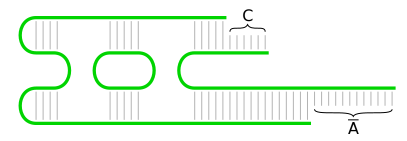
\includegraphics[width=\textwidth]{./figures/tile_model/DNA_struct.pdf} % 115mm
		\caption{Corner DAE unit}
		\label{fig:DNA_struct}
	\end{subfigure}%
	%add desired spacing between images, e. g. ~, \quad, \qquad etc.
	%(or a blank line to force the subfigure onto a new line)
	\begin{subfigure}[b]{0.472\textwidth}
		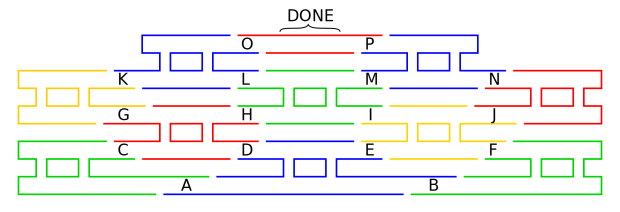
\includegraphics[width=\textwidth]{./figures/tile_model/DNA_assembly.pdf} % 175mm
		\caption{Whole self-assembly}
		\label{fig:DNA_assembly}
	\end{subfigure}
	\begin{subfigure}[b]{0.190\textwidth}
		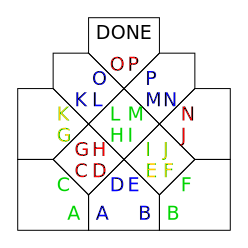
\includegraphics[width=\textwidth]{./figures/tile_model/abstract_model.pdf} % 70mm
		\caption{Abstract model}
		\label{fig:abstract_model}
	\end{subfigure}
	\caption{Evolution of abstract model from DAE units to tiles.}
	\label{fig:evolution}
\end{center}
\end{figure}
